\chapter{Specification and system design}
\label{spec}
The final system consists of three main stages: data collection, face detection
and classification, which also includes pre-processing and feature-selection.

\begin{figure}
\begin{center}
    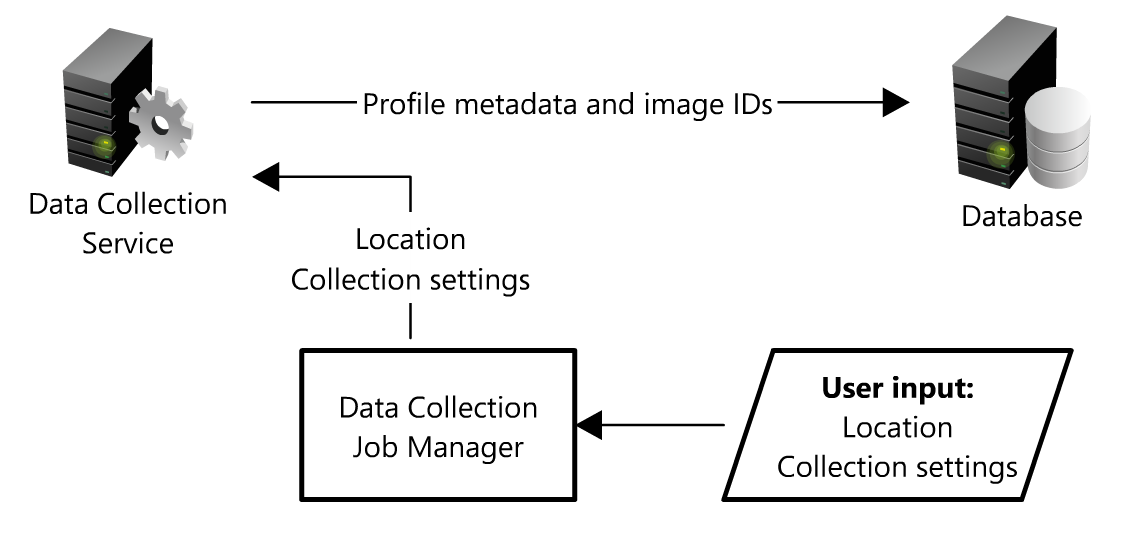
\includegraphics[width=\textwidth]{figures/spec/diagram_collection}
\end{center}
\caption{Structure of the data collection part of the system.}
\label{fig:spec:diagram_collection}
\end{figure}

In data collection there is one main component whose aim is to collect location
data and pictures of users on a mobile dating service called Tinder. User
profile metadata is saved in a relational database while images are saved to
disk. This component provides an interface to control how the data is collected
and from which locations. This interface is used by a command line utility
called Data Collection Job Manager (DCJM) which makes it easy to control the data
collection process.

\begin{figure}
\begin{center}
    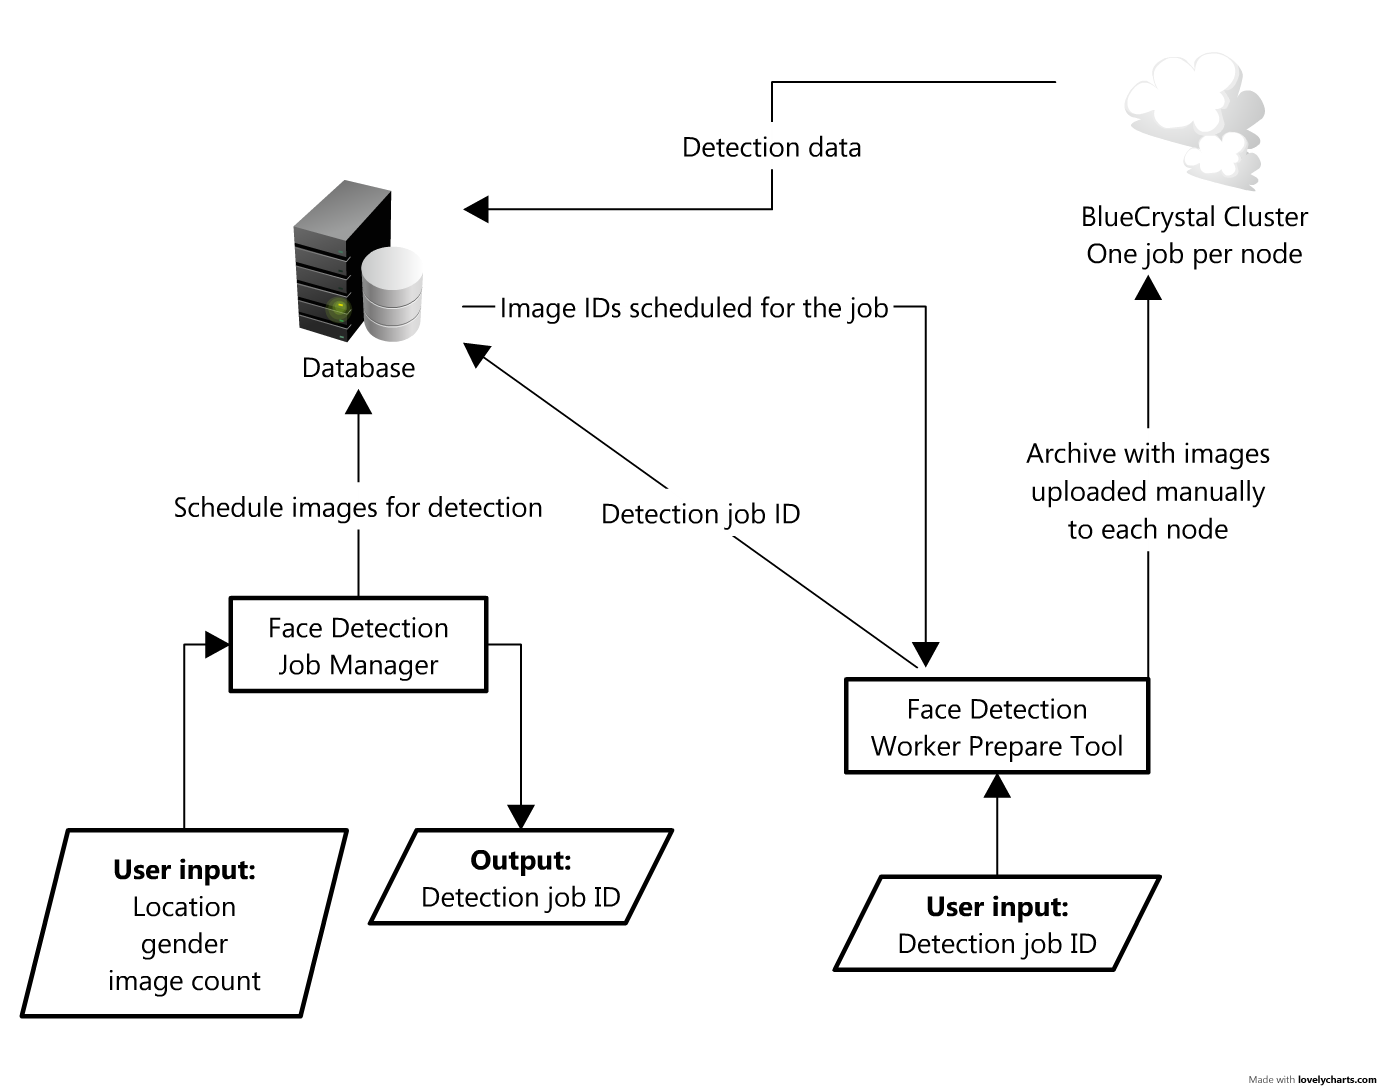
\includegraphics[width=\textwidth]{figures/spec/diagram_detection}
\end{center}
\caption{Structure and interaction of face detection components. The actual
face detection algorithm runs in the cluster on individual nodes. The database
in this diagram is the same as in Figure \ref{fig:spec:diagram_collection}.}
\label{fig:spec:diagram_detection}
\end{figure}

The main component of the face detection stage is a C++ implementation of a
novel face detection algorithm which outperforms common algorithms in the area
such as Viola-Jones and mostly matches the accuracy of the best commercial face
detection systems such as those used by Google Picasa and face.com. The output
of this component includes a rough viewpoint estimation, locations of landmarks
and a score that tells us about the quality of the detection. This data is
saved to the same database as the data collection service.

Despite impressive accuracies achieved in benchmarks using MultiPIE and
Annotated Faces in the Wild (AFW), it has one significant downside. The time
taken to detect one or more faces in a picture averaged at around 7 seconds,
which was a serious obstacle since thousands of pictures needed to be analysed
for faces.

In order to mitigate this factor a set of tools was implemented so that the
process of detecting faces in thousands of pictures becomes as modular as
possible. As a result, a concept of detection jobs was introduced so that images
could be processed in parallel on several machines.

Face Detection Job Manager (FDJM) is a tool which is similar to
DCJM\footnote{Data Collection Job Manager} and provides a command line
interface to select images to go through the face detector. The output of this
tool upon a successful creation of a detection job is a numeric ID of the job.
This ID can then be provided to the Face Detection Worker Prepare tool which
creates an archive with the required files to be processed by the face detector
component on a dedicated remote machine.

\begin{figure}
\begin{center}
    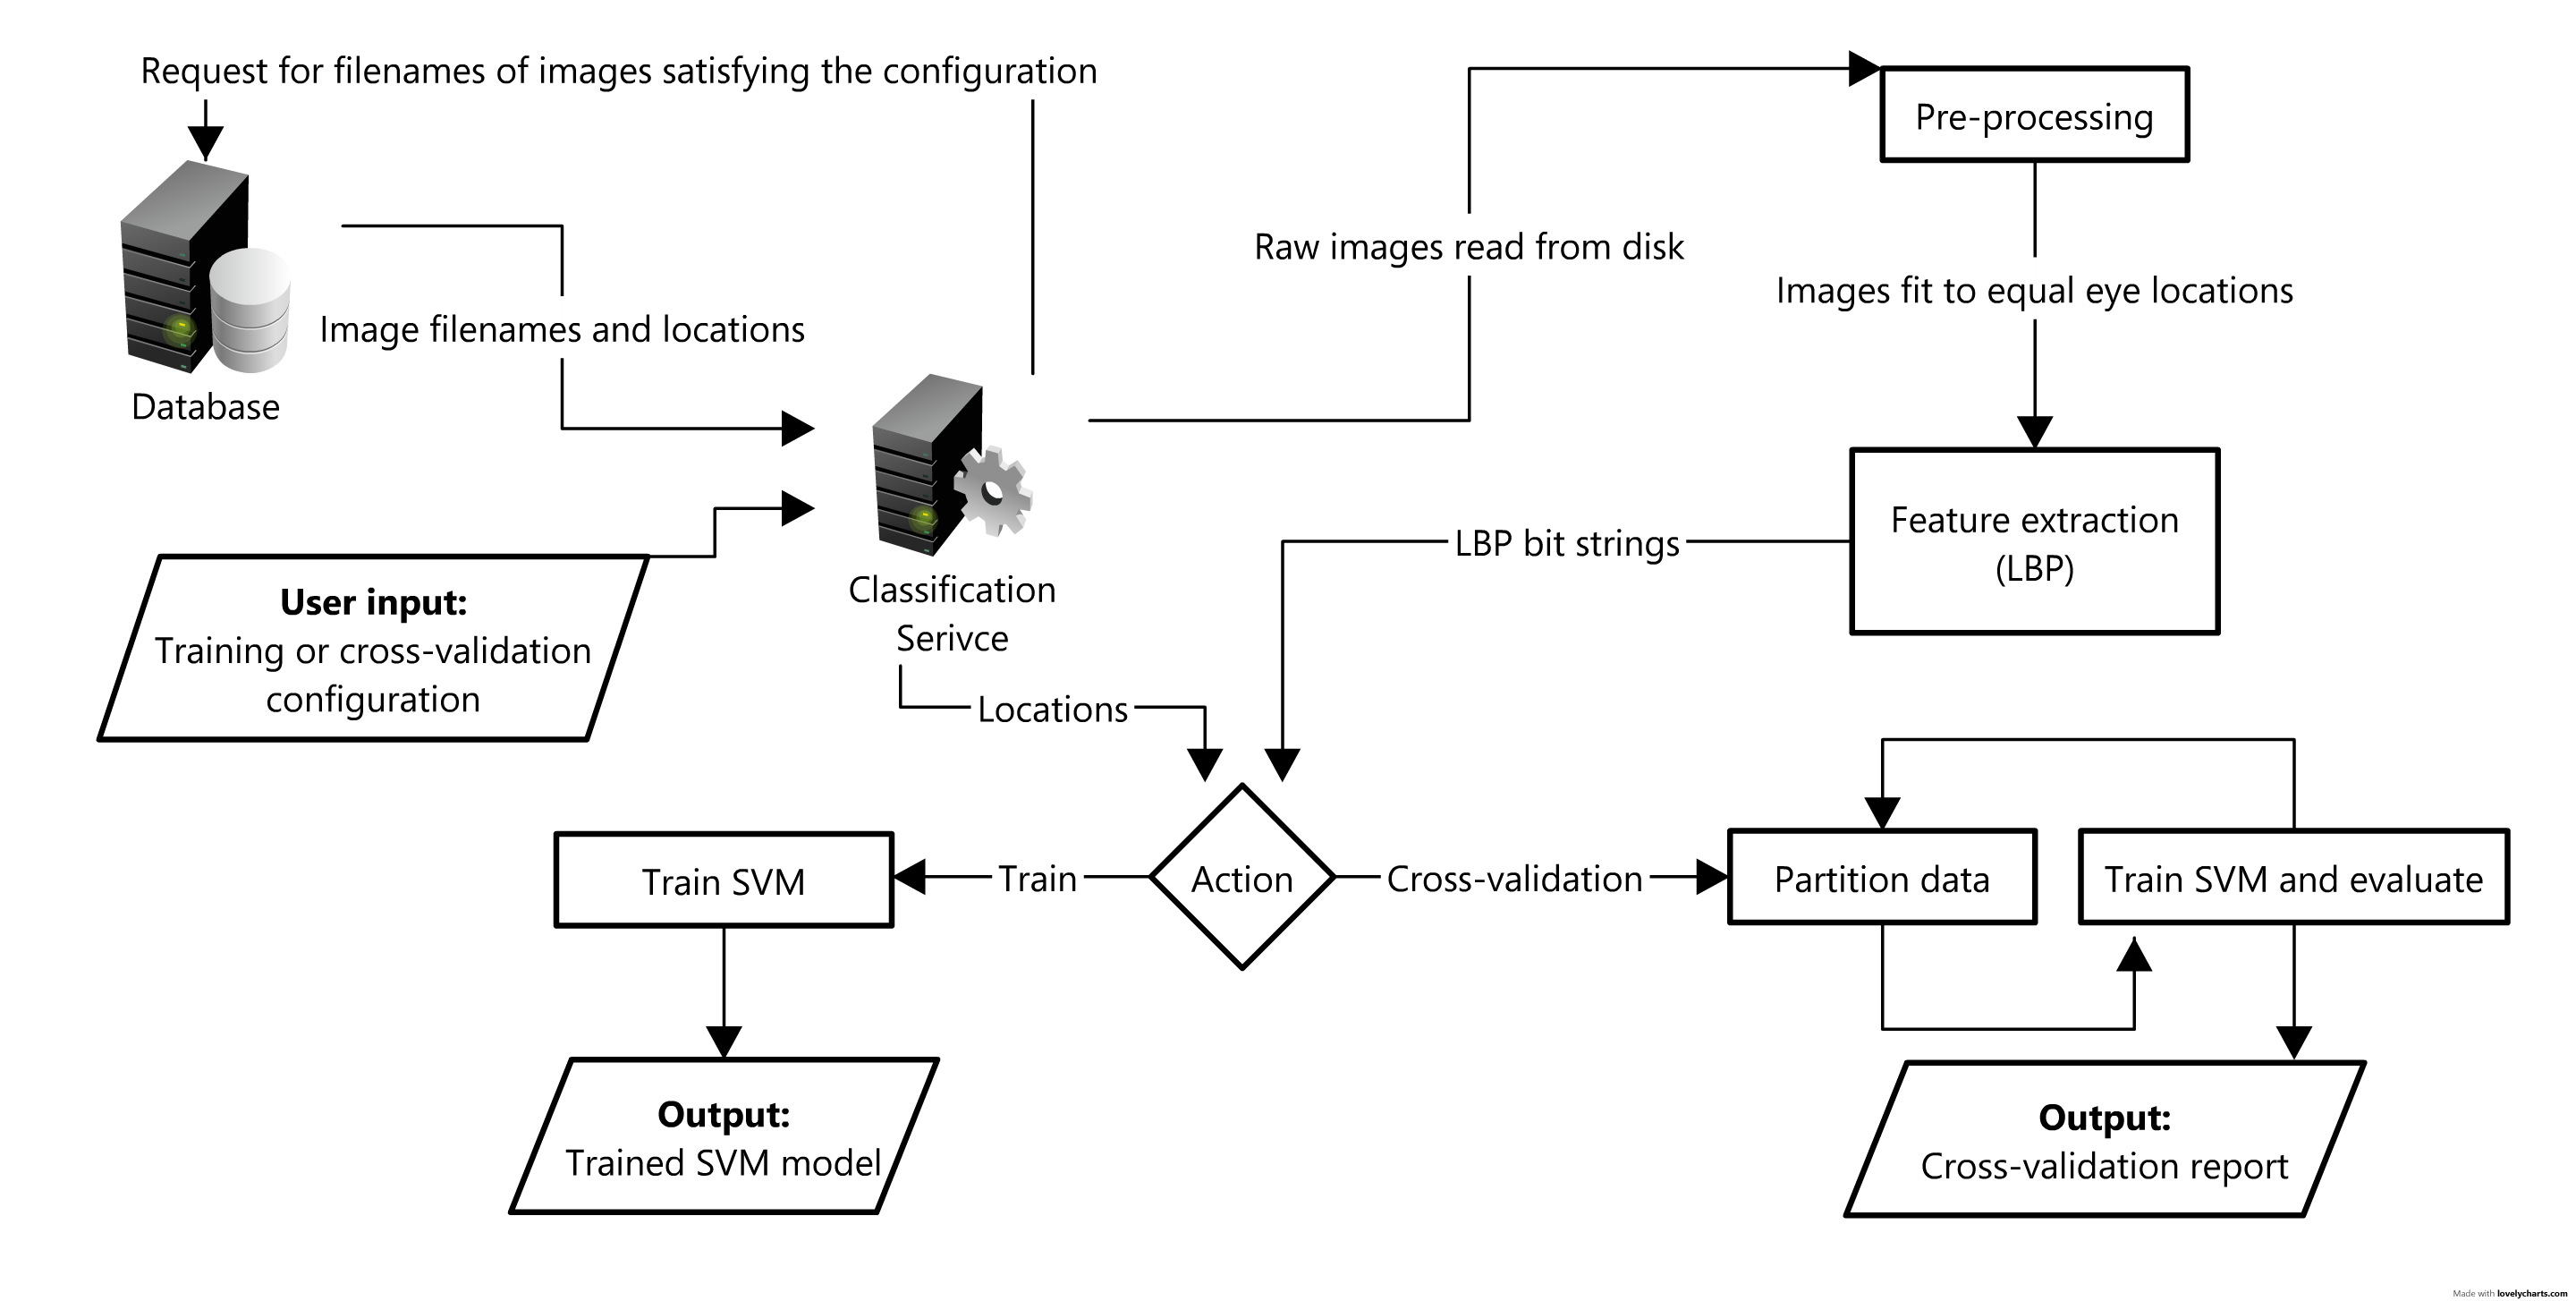
\includegraphics[width=\textwidth]{figures/spec/diagram_classification_cvtrain}
\end{center}
\caption{Part of the classification stage which is used to perform
cross-validation to find the best features, classifier and classifier
parameters. The database in this diagram is the same as in Figures
\ref{fig:spec:diagram_collection} and \ref{fig:spec:diagram_detection}.}
\label{fig:spec:diagram_cvtrain}
\end{figure}

\begin{figure}
\begin{center}
    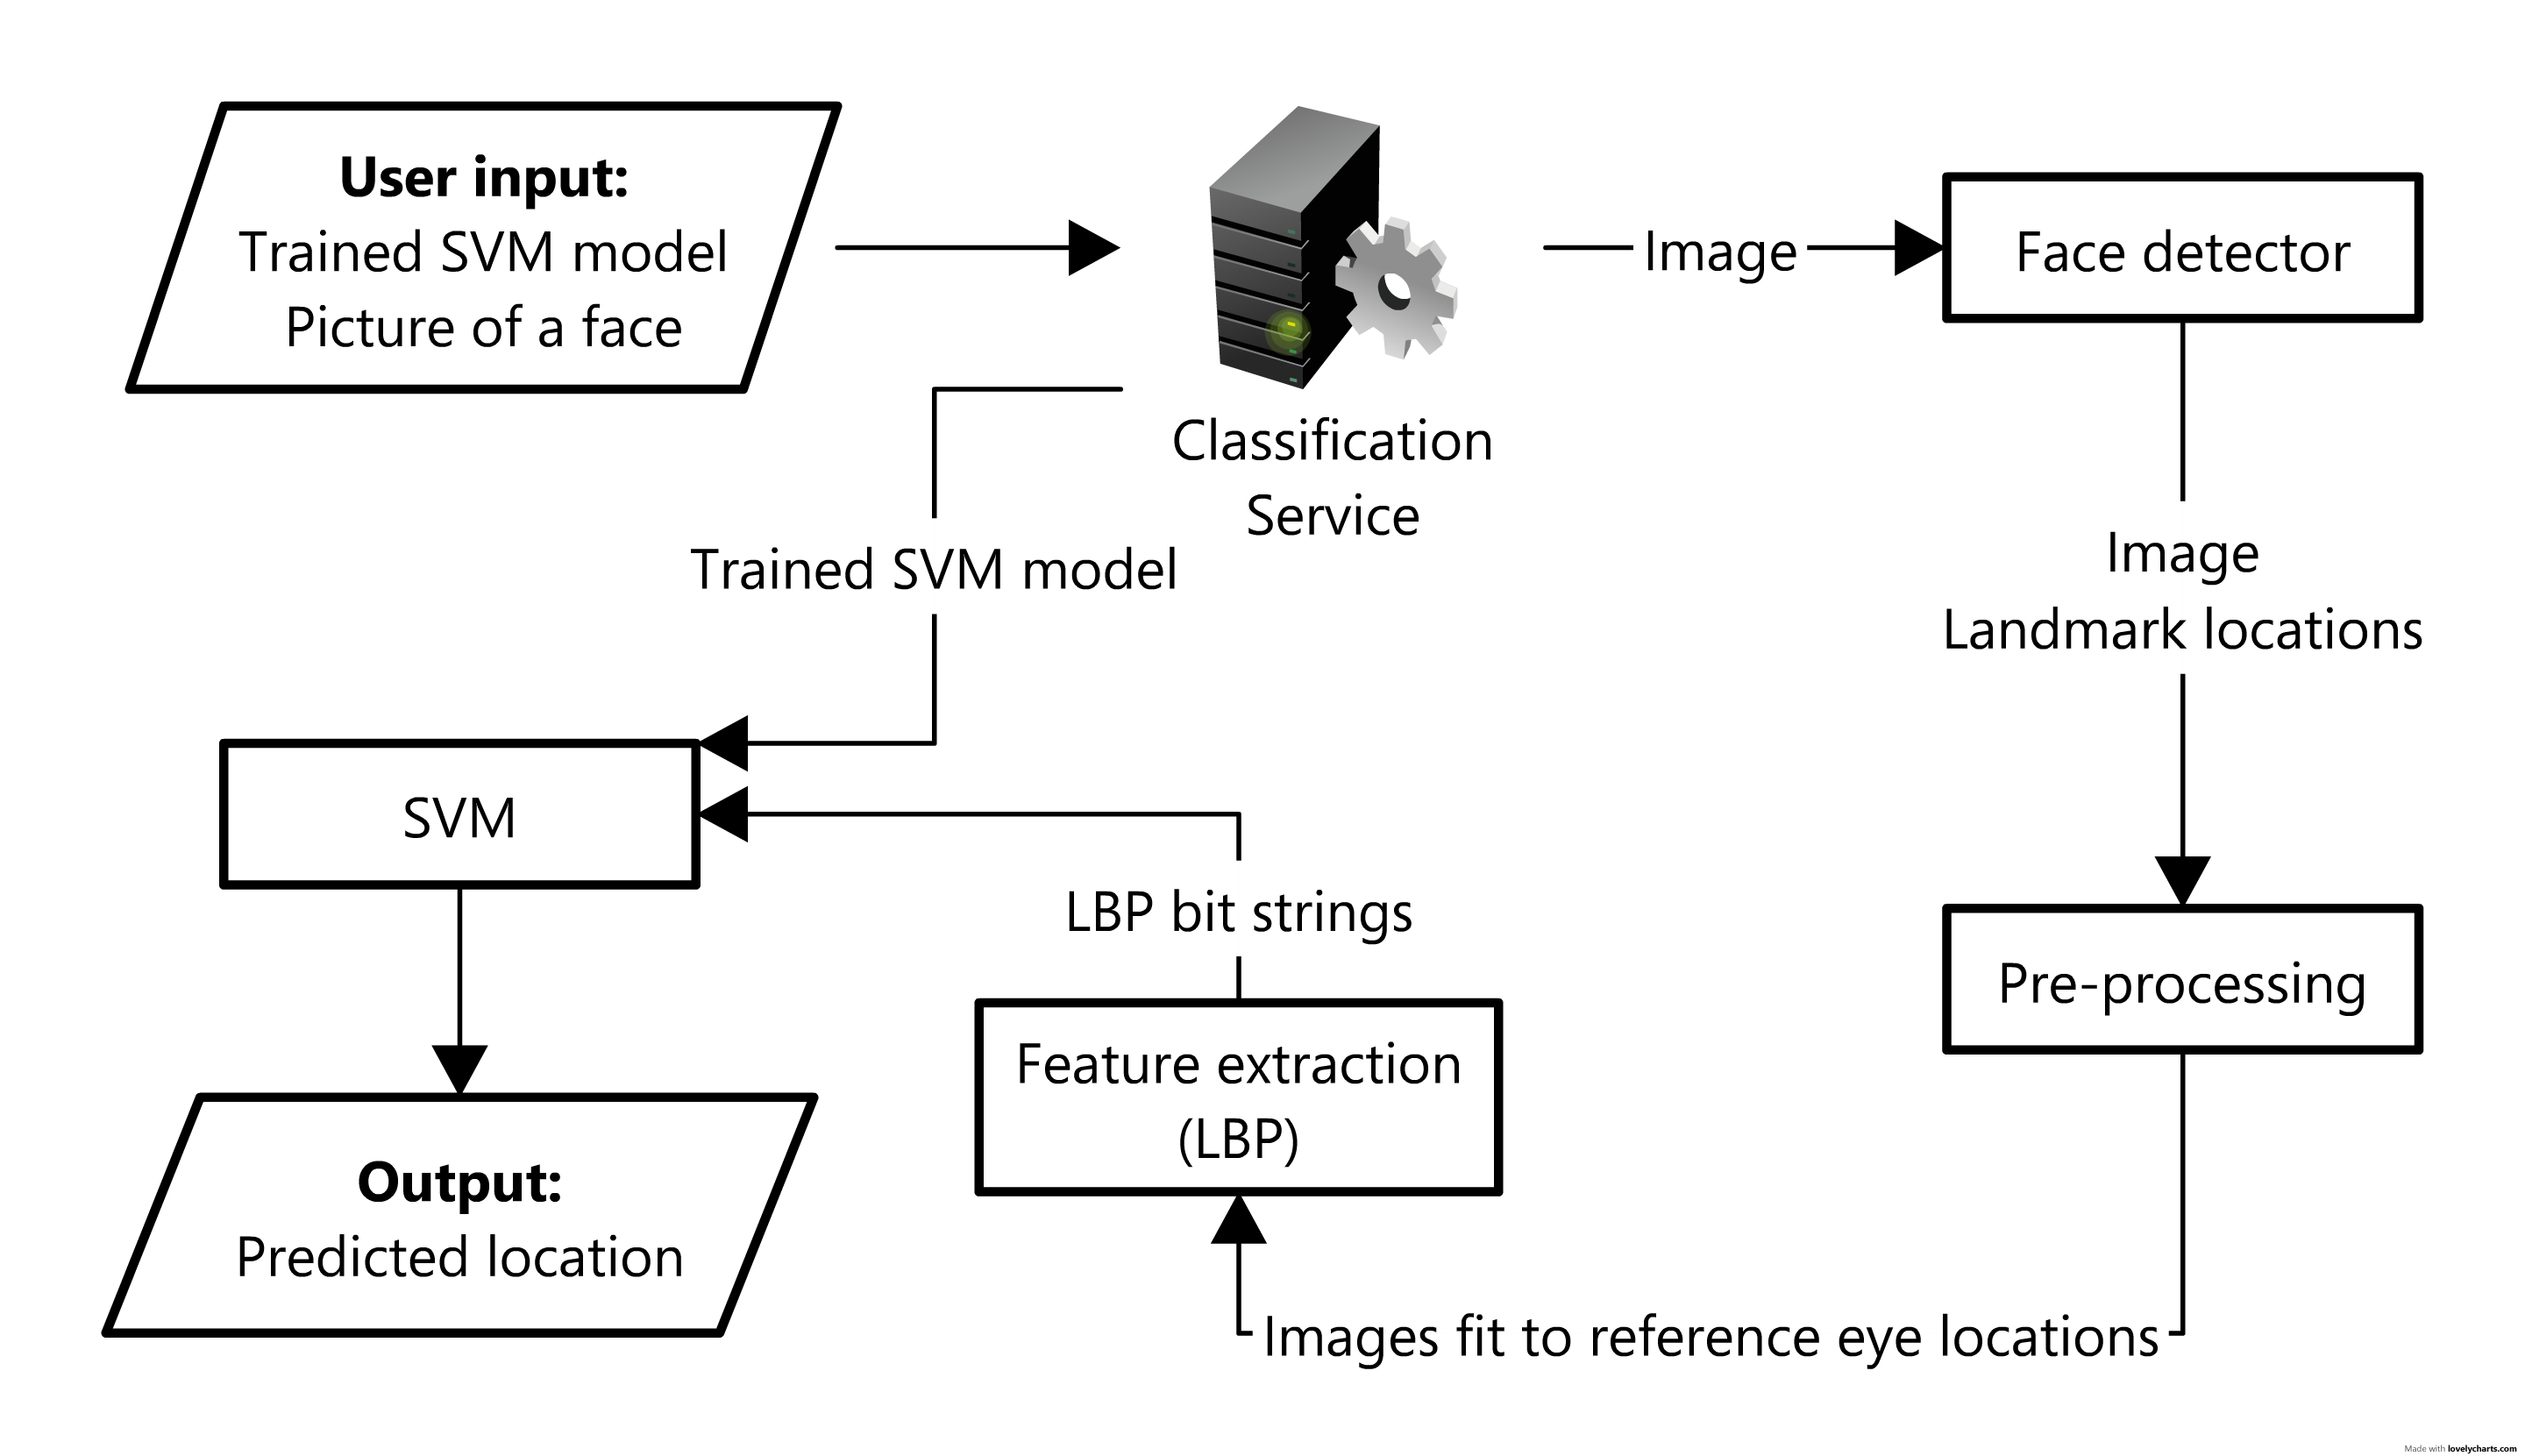
\includegraphics[width=\textwidth]{figures/spec/diagram_classification_classify}
\end{center}
\caption{The same component can also be used to estimate the person's location
from a picture of their face.}
\label{fig:spec:diagram_classify}
\end{figure}

Finally, the last stage incorporates several components responsible for
training a classifier that can estimate a person's location from a picture of
their face using the collected images and face detection results from previous
stages.

Pictures collected on Tinder were taken at a variety of angles and scales,
making it hard to detect patterns when looking at the data as a whole. In order
to eliminate these factors from the dataset all images are rotated, scaled and
aligned so that the eyes always appear in the same location in the image. This
is a simple task as the face detector results include the locations of both
eyes. Since we have the actual eye positions and the target eye positions it is
possible to calculate the angle, scale and translation factors needed to build
a transformation matrix and apply affine transform. The transformation is the
output of the Pre-processing step (Figure \ref{fig:spec:diagram_classify}). 

Next, features are extracted using local binary patterns and used in
combination with user location data obtained in the data collection stage to
train a support vector machine.

The \texttt{classification} tool provides options to train a single model to be
used when classifying novel images and to perform cross-validation according to
a configuration file with various parameters.


\section{Data collection}
The quantity and the quality of training data is crucial to all computer vision 
projects. However, for this task there was no luxury of using an existing 
dataset with the required level of detail in labels that would also be 
affordable.

A decision was made to collect own data for this project from a social network 
that makes it easy to associate user profiles with photos of themselves with 
locations accurate to city-level. Popular social networks such as Facebook 
would be ideal for this, however it is not possible to obtain a list of 
profiles from a hand-picked location due to Facebook API constraints. 
Moreover, it is clearly stated in Facebook's Terms and Conditions that any way 
to circumvent these constraints would still count as a violation.


\subsection{Tinder}
Tinder is a mobile dating application that shows profiles closest to the 
user's GPS location. There have been numerous third-party Tinder utilities on 
the Web that reverse-engineered Tinder's simple and unobfuscated HTTP API that 
makes it possible to create a fully-featured Tinder client yourself.

The API has support for various actions such as liking and messaging users, 
but for the purposes of this project, the only relevant actions to us are 
authentication, setting own location using latitude and longitude coordinates 
and fetching nearby users.

Tinder profiles are created using Facebook Login. When the application is 
opened for the first time by a non-registered user, they will be prompted to 
login using their Facebook account which gives Tinder access to the user's full name, 
age, pictures and other details.

A user profile was created specifically for this project using the original 
Tinder mobile application on an Android phone. 

\subsection{Profile metadata and photo collection}
A web application (\texttt{tinder-gather}) was written to mimic the Tinder app
whose only purpose was to record profile metadata such as name, location and
date birth as well as to save user-uploaded pictures. 

This web application provides an API that allows an external tool 
(\ref{spec:data:jobs}) to easily change the location of the user for this 
application so that images are collected from several different 
countries.

The web application must be used with a complementary Chrome extension 
(\texttt{tinder-gather-connect}) that handles Facebook authentication.
Once the extension is installed a button to launch the app will appear in the 
toolbar. As soon as the user signs in the app will be ready to accept data 
collection jobs from the Tinder job manager tool (\ref{spec:data:jobs}).

\subsection{Data collection and detection job manager}
\label{spec:data:jobs}
Images of people need to be collected from a number of different locations 
around the world. Specifying the coordinates of each location using latitude 
and longitude values proved to be cumbersome in the beginning which is why a 
special and user-friendly tool was written to manage data collection from the 
command line.

This tool resides in the \texttt{tinder-gather} project in the \texttt{tools} 
directory. Usage and help will be displayed in the terminal if ran with these 
arguments:
\begin{logs}
./jobs.js tjob post
\end{logs}

This command expects three arguments: location, limit and delay. Location is 
just a city name whose location is hard-coded inside the script and can be 
easily extended. This argument is required. Limit refers to the maximum number 
of profiles to fetch from Tinder at once and delay specifies how frequently 
they will be fetched.

When a job is created and the data collection service is notified it starts
collecting user profile metadata and their pictures. The profile metadata is
saved into a database along with the filenames of images that are stored on
disk in a single directory.

This tool is also used to manage face and landmark detection jobs which will 
be described in detail in Section \ref{spec:fd}. 

\section{Face and landmark detection}
\label{spec:fd}
Before the collected pictures of faces from different parts of the world 
could be used to learn how to determine the location of a person from a single 
picture of their face they must first be heavily filtered as many Tinder users 
upload very low-quality pictures or even pictures of pets and inanimate 
objects.

A face detector is an ideal method of filtering out non-face images as well as
heavily edited or poor quality face pictures. 

Viola-Jones is the most popular choice for face detection due to its 
incredible performance and native implementation in OpenCV, but it falls 
behind some other face detection algorithms such as those used by 
Google Picasa and face.com.

Unfortunately, Google Picasa and face.com use closed-source 
solutions making them unsuitable for use in this project. However, it was 
discovered that there is an open face detection model that comes very close 
to these commercial algorithms and significantly outperforms Viola-Jones at
the face detection task.

The model can also be trained to learn landmark localisation and face angle, 
which provide additional information that enables us to further filter and 
pre-process the images collected from Tinder profiles. This is important 
because being able to estimate the locations of certain landmarks such as eyes 
makes it possible to scale and rotate images so that the landmarks line up.

Another advantage of this particular solution is that it comes with 
pre-trained on the MultiPIE dataset which otherwise would need to be purchased. 

\subsection{Face, landmark and pose detection using mixture of trees and HoG}

In this model, there is a shared pool of facial landmarks encoded as parts and denoted $V$.
Every viewpoint is modelled as a tree-structured pictorial structure $T_m = (V_m, E_m)$
where $E_m$ is a set of edges and $V_m \in V$.

The locations of each part ($L = {l_i : i \in V}$) can be scored as follows:
\begin{flalign}
    \label{eq:spec:fd:S}
    S(I,L,m) = \text{App}_m(I,L) + \text{Shape}_m(L) + \alpha^m 
\end{flalign}

\begin{flalign}
    \label{eq:spec:fd:App}
    \text{App}_m(I,L) = \sum_{i \in V_m} w_i^m \cdot \phi(I,l_i) 
\end{flalign}

\begin{flalign}
    \label{eq:spec:fd:Shape}
    \text{Shape}_m(L) = \sum_{ij \in E_m} a_{ij}^m dx^2 + b_{ij}^m dx + c_{ij}^mdy^2 + d_{ij}^m dy 
\end{flalign}

Equation \ref{eq:spec:fd:App} computes the appearance evidence of part $i$
using template $w_i^m$ which is tuned for mixture/viewpoint $m$. $\phi(I,l_i)$
is the feature vector (e.g. Histogram of oriented gradients) at location $l_i$
of image $I$.

In Equation \ref{eq:spec:fd:Shape} $dx = x_i  - x_j$ and $dy = y_i - y_j$
correspond to $x$ and $y$ displacements of part $i$ relative to part $j$. "Each
term in the sum can be interpreted as a spring that introduces spatial
constraints between a pair of parts, where the parameters $(a,b,c,d)$ specify
the rest location and rigidity of each spring." \citep{zhu2012face}
The $\alpha^m$ term refers to the bias of viewpoint mixture $m$. 

The score from equation \ref{eq:spec:fd:S} was used to determine which face 
detection results were the most reliable and suitable for this project.

The objective of the learning stage is to maximise $S(I,L,m)$ in Equation
\ref{eq:spec:fd:S} over $L$ and $m$, i.e:
\begin{equation}
\label{eq:spec:fd:maxS}
S^*(I) = \max_m[\max_L S(I,L,m)]
\end{equation}

Equation \ref{eq:spec:fd:maxS} says that for every mixture/viewpoint we find
the best set of part/facial landmark locations $L$ as scored by Equation
\ref{eq:spec:fd:S} and then choose the mixture with the highest score received.
Maximisation over $L$ is performed using dynamic programming.

\improvements[inline,caption={}]{
        Subsections I can expand on:
        \begin{itemize}
            \item Learning specifics
            \item Results/performance comparison with other face detection
                systems (including Viola-Jones)
        \end{itemize}
}

There is a total of 13 viewpoints ranging from $-180^\circ$ to $180^\circ$ in
$15^\circ$ increments. For frontal face pictures, where the viewpoint is
between $-45^\circ$ and $45^\circ$, there are 68 landmarks and 39 landmarks for
other, profile viewpoints. When we detect a face using this algorithm we also
obtain the set of landmark locations $L$ and an approximate viewpoint.

The majority of pictures collected for this project fall into the frontal
category and convey more information than profile pictures so only those will
be used.

Landmark points are placed on faces such that they outline the nose, eyes,
mouth, jaw and the overall shape of the face. The particular groups of landmark
locations are specified in Table \ref{table:spec:fd:landmarks}.

\begin{wraptable}{r}{5.5cm}
    \begin{tabular}{cc}\\\toprule  
        Face part & Landmark range \\\midrule
        Nose      & 1-9 \\  \midrule
        Left eye  & 10-15 \\  \midrule
        Right eye & 21-26\\  \midrule
        Mouth     & 32-51 \\  \bottomrule
    \end{tabular}
    \caption{A wrapped table going nicely inside the text.}
    \label{table:spec:fd:landmarks}
\end{wraptable} 

To summarise, when this algorithm detects a face in a picture it outputs the 
locations of important landmarks, face angle to the nearest $15^\circ$
increment and score to say how accurate the detection is.

\subsection{Face detection component}
This face detection algorithm functions as a separate component which is
comprised of a face detection job manager and a single executable which
performs face detection using this algorithm.

The executable takes a list of image filenames as standard input and loads a
configuration file which contains the name of the directory where all images
are saved during data collection. After ensuring that all the images exist on
disk it starts performing face detection on each image one-by-one and saving
the output of the algorithm: the locations of landmarks, face angle and score,
to a database.

Creating a list of image filenames to process was cumbersome so the Tinder job
manager tool introduced in \ref{spec:data:jobs} was extended to support
creating such lists. 

Usage information for this job action can be displayed by running the following
command:
\begin{logs}
./jobs.js djob post
\end{logs}

In order to create a list of images to process the user must specify the
location of Tinder profiles whose images will be retrieved, gender and the
number of images to put in the list. If ran successfully, this will schedule
the images retrieved according to the specified filters to be processed as a
detection job whose numeric ID will be given as the output.

Compared to remarkably impressive speed performance of Viola-Jones, this
particular algorithm can take on average around 7 seconds to process a single
picture. This led to the face detection component being designed to run as
lock-free, concurrent instances with each having its own job ID so that it can
run on multiple machines at the same time.

A tool located in the \texttt{detect-worker} repository under the name
\texttt{prepare-detect-worker} was written to create \texttt{tar} archives
which contain the necessary image files needed for a particular detection job.
The tool takes a detection job ID as the only argument and creates an archive
with filename \texttt{job-<ID>.tar} which should be uploaded to the machine
that will be used to run this face detection job.

On the target machine the user must run \texttt{prepare-job} in the same
directory as the \texttt{job-<ID>.tar} archive and the face detector
executable. The face detection executable loads a configuration file which
contains the hostname and credentials for the remote database server used by
the data collection service. This is needed because the face detector will save
detection results to that remote server.

\section{Data analysis and classification}
\improvements[inline,caption={}]{Everything mentioned here is actually
implemented in a single script. I can talk about how these components interact
inside it.}

\unsure[inline]{I have tried many pre-processing techniques, feature extraction
methods and classifiers. Should I only mention my final choices or not mention
the particular algorithms I have used at all?}


\subsection{Pre-processing}
\label{spec:preproc}
\newcommand{\vleftright}{\vec{v}_i^{\text{left} \rightarrow \text{right}}}
\newcommand{\vi}[1]{\vec{v}_i^{\text{#1}}}
\newcommand{\vr}[1]{\vec{v}_{\text{ref}}^{\text{#1}}}
\newcommand{\vref}{\vec{v}_{\text{ref}}^{\text{left} \rightarrow \text{right}}}
The problem with using unprocessed Tinder profile pictures is that they are 
taken at a variety of different angles and scales. Before these pictures can 
be used to train a classifier they must first be transformed so that they all 
have the same angle and scale. This was done by using previously detected 
locations of eyes as reference points so that they always appear in the same 
location in the image. 

Throughout this section $\vi{left}$ and $\vi{right}$ will refer to the
coordinates of the left and right eyes, respectively, in the original image.
Vector $\vleftright$ passes through the locations of detected eyes in the image
and is defined as $\vleftright = \vi{right} - \vi{left}$. Vectors
$\vr{left}$ and $\vr{right}$ are our target eye locations to which all images
will be mapped.

Computing a rotation matrix is the first step in performing an affine transform
to ensure that all faces have the same rotation and scale. Before it can be 
computed we must first calculate the rotation angle $\theta$, scaling factor
$s$ and centre of the rotation $\vec{c}$ in the original image.

\begin{equation}
    \label{eq:spec:preproc:angle}
    \theta = -\arccos{\frac{\vleftright \cdot \vref}{|\vleftright| |\vref|}}
\end{equation}
Angle $\theta$ is rotation of the original face relative to the target face
location and can be calculated as the angle between vectors $\vref$ and
$\vleftright$ using the definition of the dot product.

\begin{equation}
    \label{eq:spec:preproc:scales}
    s = \frac{|\vref|}{|\vleftright|}
\end{equation}

\begin{equation}
    \label{eq:spec:preproc:centre}
    \vec{c} = \frac{\vi{left} + \vi{right}}{2}
\end{equation}
The original image should be rotated around the midpoint of $\vi{left}$ and
$\vi{right}$.

\begin{equation}
    \label{eq:spec:preproc:mat}
    \begin{bmatrix}
    \alpha & \beta  & (1-\alpha)\cdot \vec{c}_x - \beta \cdot \vec{c}_y + \vec{t}_x \\
    -\beta & \alpha & \beta \cdot \vec{c}_x + (1-\alpha)\cdot \vec{c}_y + \vec{t}_y
    \end{bmatrix}
\end{equation}
Using the computed rotation angle and point of rotation we obtain a
transformation matrix (\ref{eq:spec:preproc:mat}) to perform this operation
using affine transform. In this equation $\alpha = s\cos\theta$ and $\beta =
s\sin\theta$. An additional translation vector ($\vec{t}$) was added to the
third column in this matrix to move the midpoint of the eyes in the image to
the same location as the midpoint of the reference eye locations (Equation
\ref{eq:spec:preproc:midtr}). 

\begin{equation}
    \label{eq:spec:preproc:midtr}
    \vec{t} = \frac{\vi{left} + \vi{right}}{2} - \frac{\vr{left} + \vr{right}}{2}
\end{equation}
After this transformation the distance between eyes and their locations
($\vi{left}$ and $\vi{right}$) should match the reference eye locations
($\vr{left}$ and $\vr{right}$).
\unsure[inline]{Should I put here step-by-step snapshots of face
transformation? For example: original, rotated, scaled, translated.}
\unsure[inline]{Alternatively, I could do the same with a graph and vectors
representing the eyes.}

\subsection{Feature extraction}
\improvements[inline,caption={}]{Short section stating that LBP (local binary
patterns) was used and parameters. I can explain how it works with
illustrations.}

\subsection{Classification}
\improvements[inline,caption={}]{
    \begin{itemize}
        \item cross-validation tool to compare feature pre-processing,
            extraction methods, classifiers and their parameters.
        \item training
    \end{itemize}
}

%%% Local Variables: 
%%% mode: latex
%%% TeX-master: "thesis"
%%% End: 
